\chapter[Simulating Fuel Cycles]{Simulating Fuel Cycles}
\section{Simple Verification}
In this work, several demonstration simulation verified the capabilities implemented in Pyre. \Cyclus archetypes are expected to meet a number of capabilities such as trading, decommissioning, and isotope tracking.
To demonstrate these functionalities we ran a simple scenario with one source, sink, and Pyre facility. The Pyre facility is run at default values 
corresponding to an average installation. The source facility provides light water reactor (LWR) SNF with a composition given by Duderstadt \cite{duderstadt_nuclear_1976}. 

\FloatBarrier

\begin{figure} [h]
	\centering
	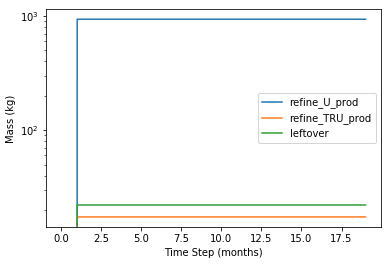
\includegraphics[width=0.65\linewidth]{images/timeseries-prod}
	\caption{Product time series of a simple simulation.}
	\label{fig:timeseries-prod}
\end{figure}



\begin{figure} [h]
	\centering
	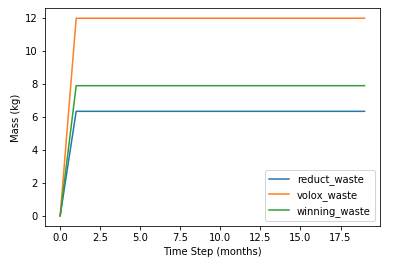
\includegraphics[width=0.65\linewidth]{images/timeseries-waste}
	\caption{SNF in the Pyre facility for the simplest simulation.}
	\label{fig:timeseries-waste}
\end{figure}

The above Figures \ref{fig:timeseries-prod} and \ref{fig:timeseries-waste} track the shipment of the LWR SNF from the Pyre facility to the \texttt{sink}.
Individual waste streams are identified and verify the functionality of each sub-process in this LWR configuration. Since the scenario was run with
constant sub-process parameters and a constant number of facilities, the transactions are expected to remain constant and the above figures meet this expectation.
In addition to demonstrating sub-process capabilities, material transactions with other \Cyclus facilities can also be observed as expected. Material trade is verified by the continual separation of SNF without a buildup of waste or product.

\subsection{Isotopic Streams}
\begin{figure} [h]
	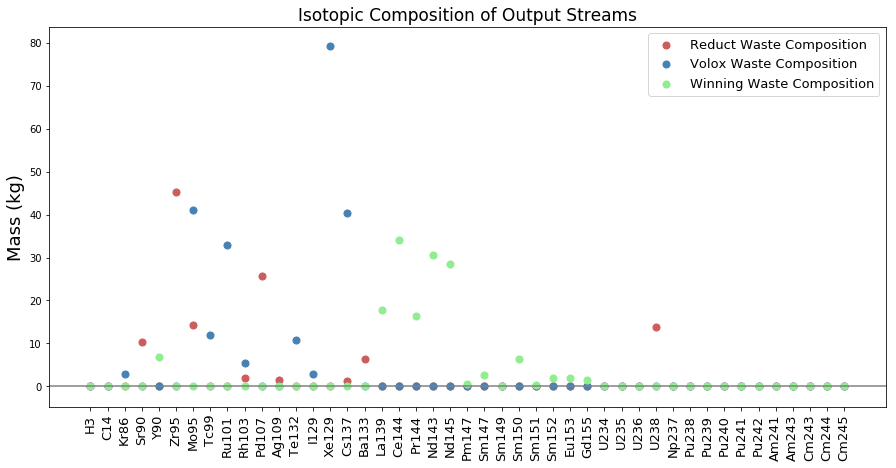
\includegraphics[width=\linewidth]{images/avg-isotope-comp}
	\caption{Isotopic composition of average waste streams}
	\label{fig:avg-isotope-comp}
\end{figure}

Another key aspect of material transactions is the composition of each shipment. To meet \Cyclus standards Pyre must be able to track each isotope and trading with various facilities. This is done two ways within Pyre: monitoring waste and product transactions, and tracking isotopic compositions.
Figure \ref{fig:avg-isotope-comp} compares three waste streams isotopically. This comparison further illuminates the performance of each sub-process by confirming the appropriate separation of elements.
The electrowinner, shown in green, correctly contains heavier elements such as lanthanides while the electroreductor, in red, is responsible for the lighter metals
as well as changing oxidation states which is not reflected in these streams.

\subsection{Simple Diversion}
\begin{figure} [h]
	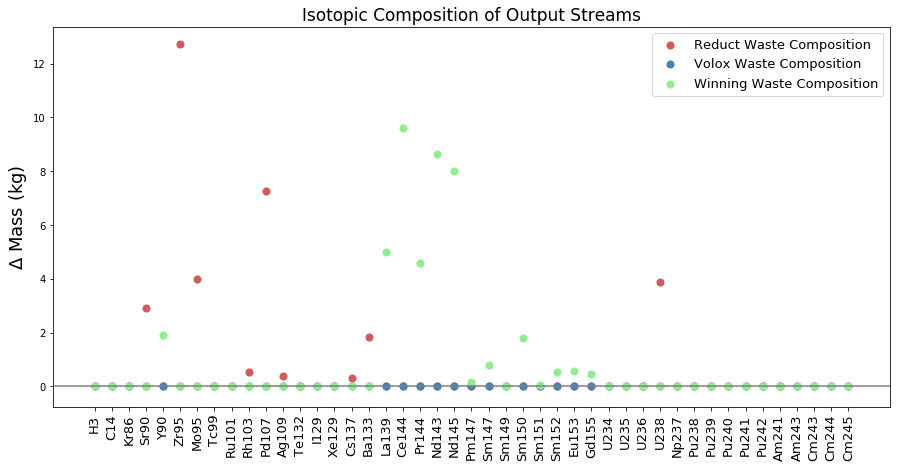
\includegraphics[width=\linewidth]{images/current-isotope-comp}
	\caption{Isotopic composition of current diverted waste streams}
	\label{fig:current-isotope-comp}
\end{figure}

\begin{figure} [h]
	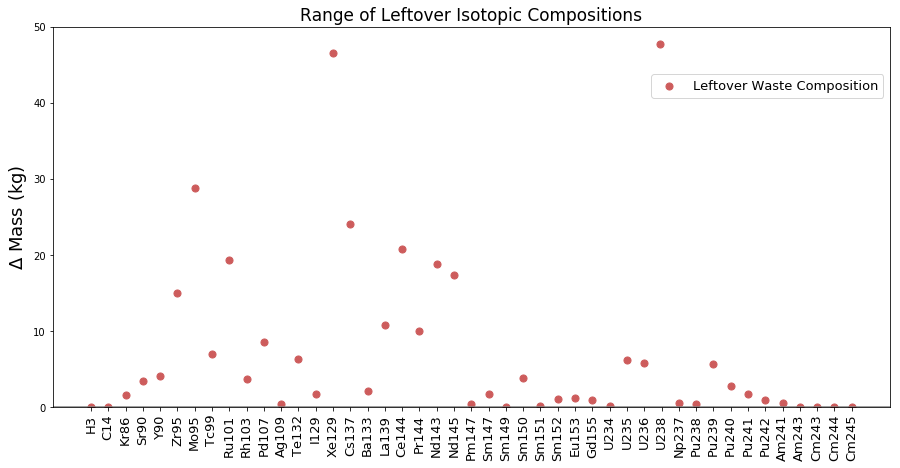
\includegraphics[width=\linewidth]{images/isotopic-comp-range}
	\caption{Range of isotopic values for maximum potential diversion.}
	\label{fig:isotopic-range}
\end{figure}

Simple diversion cases are handled through two example scenarios. The first scenario describes a facility that operates at a higher than reported current, leading to increased power draw. The second case imagines a facility diverting as much material as possible by reporting a low efficiency and operating at optimal levels.
Figures \ref{fig:current-isotope-comp} and \ref{fig:isotopic-range} are used to demonstrate these simple diversion scenarios. In particular, the scenario run for Figure
\ref{fig:current-isotope-comp} compares a facility of default values with one of increased power draw. Increasing the power draw of the facility affects sub-process currents.
Separation efficiency of the electroreductor and electrowinner is improved by increasing the current in the anode resulting in the material unaccounted for (MUF) shown above. Despite no change, the voloxidation stream
remains to confirm only appropriate processes are being affected. 

\subsection{Maximum Diversion}
The other diversion case explored here is a theoretical maximum diversion scenario in which two scenarios are run: where parameters are set to their maximum and minimum values
respectively. Although unrealistic since diversion is easily detected, the scenario shows us the worst case and can be used to inform inspection intervals.
Figure \ref{fig:isotopic-range} shows that after a 20 month scenario, approximately a significant quantity of plutonium is unaccounted for. As such, inspections would need to occur
at a similar interval, depending on the reported capacity.

\section{US Fuel Cycle Transition}

After testing the capabilities of Pyre in a steady state scenario, we implemented the archetype in the EG01-EG24 transition scenario described in the goals of this work. 

\begin{table}[h]
	\centering
	\begin{tabularx}{0.5\linewidth}{lcc}
		\hline
		\textbf{Details} & \textbf{Value} & \textbf{Unit} \\
		\hline \hline
		Simulation start & 1959 & years \\ \hline
		Simulation end & 2215 & years \\ \hline
		LWR Lifetime & 60 & years \\ 
		50\% of LWRs & 80 & years \\ \hline
		Transition start & 2015 & years \\ \hline
		Reprocessing Facility & PRIDE Pyre & -- \\ \hline
		New LWR lifetime & 80 & years \\ \hline
		SFR Lifetime & 80 & years \\ \hline
		SFR breeding ratio & 1.014 & -- \\ \hline
		Reprocessing Facility & INL Pyre & -- \\ \hline
	\end{tabularx}
	\caption {Transition scenario configuration parameters.}
	\label {tab:setup}
\end{table}

Table \ref{tab:setup} shows the setup for a sodium fast reactor (SFR) transition. In addition to the above information, the scenario is initiated with 200 LWRs with another 200 being deployed
in 2015 at the transition period. Two Pyre prototypes are deployed to handle the different fuel types seen in the above scenario. The PRIDE-based facility is configured to reprocess ceramic
LWR waste while the INL-based facility handles metallic SFR fuel, and is deployed after the transition. 

Figure \ref{fig:net-cap} demonstrates the deployment and decommissioning of reactors in this scenario. In order to meet the average 1\% annual power growth, additional reactors are necessary
while appropriate SFR fuel quantities are accumulated.

\begin{figure} [h]
	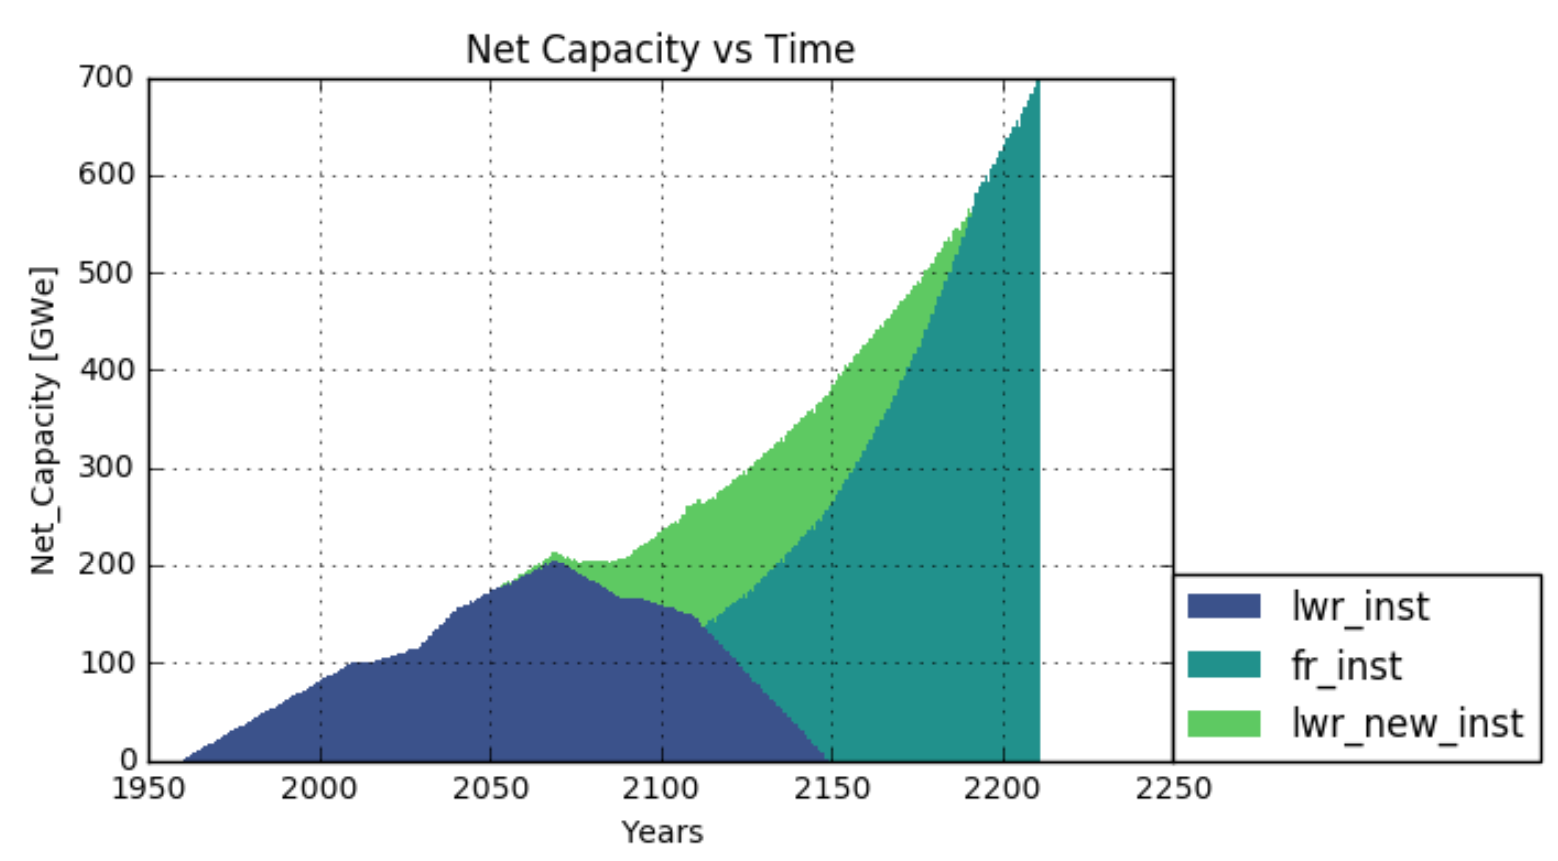
\includegraphics[width=\linewidth]{images/transition-netcap}
	\caption{Net Power Capacity over Time}
	\label{fig:net-cap}
\end{figure}

\subsection{Pyre Performance}

To verify functionality of the Pyre archetype we observe the fuel production and utilization.
Figures \ref{fig:TRU-util} and \ref{fig:u-util} demonstrate the appropriate reprocessing and fabrication of SFR fuel. Figure \ref{fig:TRU-util} shows the SFR pyroprocessing
plants begin producing a sustainable amount of fuel around year 2125. Since all SFRs are breeders in this scenario, we can see that as more reactors are deployed the TRU stock increases exponentially at year 2150. Similarly, the overall utilization of uranium improves as reprocessing is heavily used. Improved uranium utilization corresponds to the closing of the nuclear fuel cycle. The demand for uranium mining and milling diminishes as the SFR population grows causing an increase in uranium effectiveness. This is further exemplified in Figure \ref{fig:TRU-util} which illuminates the shift from enriched uranium based fuel to a TRU mix.

\begin{figure} [h]
	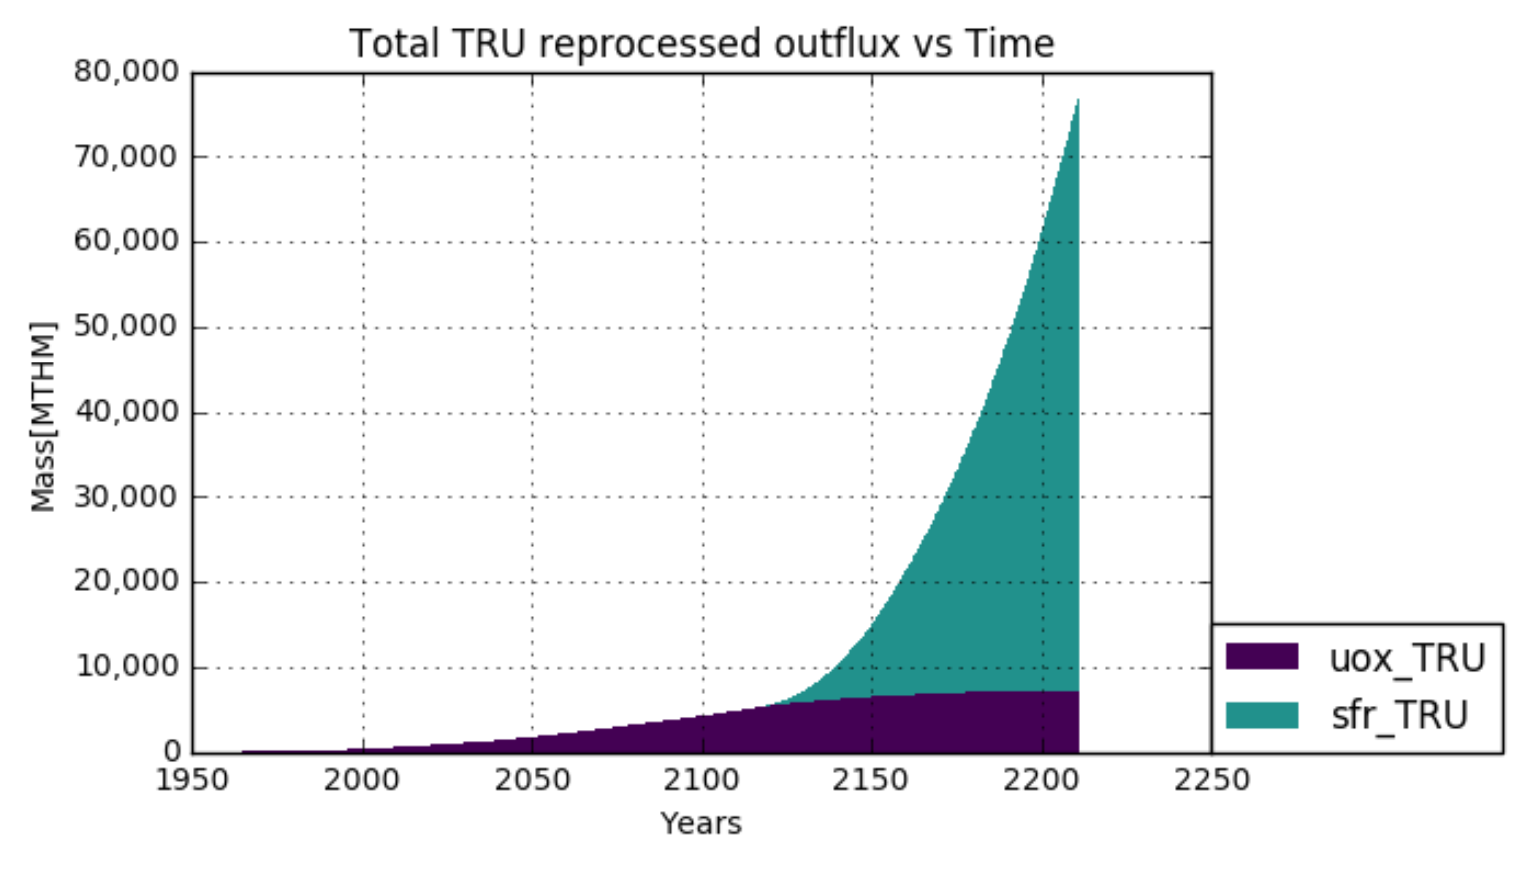
\includegraphics[width=\linewidth]{images/transition-TRUutil}
	\caption{TRU utilization over time in EG01-EG24 transition scenario.}
	\label{fig:TRU-util}
\end{figure}

\begin{figure} [h]
	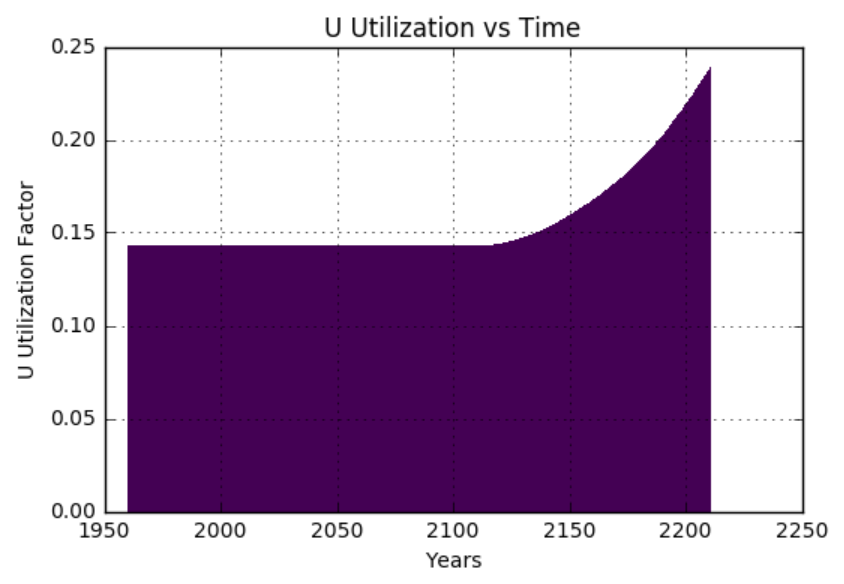
\includegraphics[width=0.8\linewidth]{images/u-util}
	\caption{Uranium utilization over time in EG01-EG24 transition scenario.}
	\label{fig:u-util}
\end{figure}

Figure \ref{fig:fuel-mass} illustrates the complete transition from LWRs and UOX fuel to SFRs at year 2180. As seen in Figures \ref{fig:TRU-util} and \ref{fig:u-util}, TRU fuel
production has increased enough to self-sustain the next generation of SFR reactors and decommission remaining LWRs.

\begin{figure}[h]
	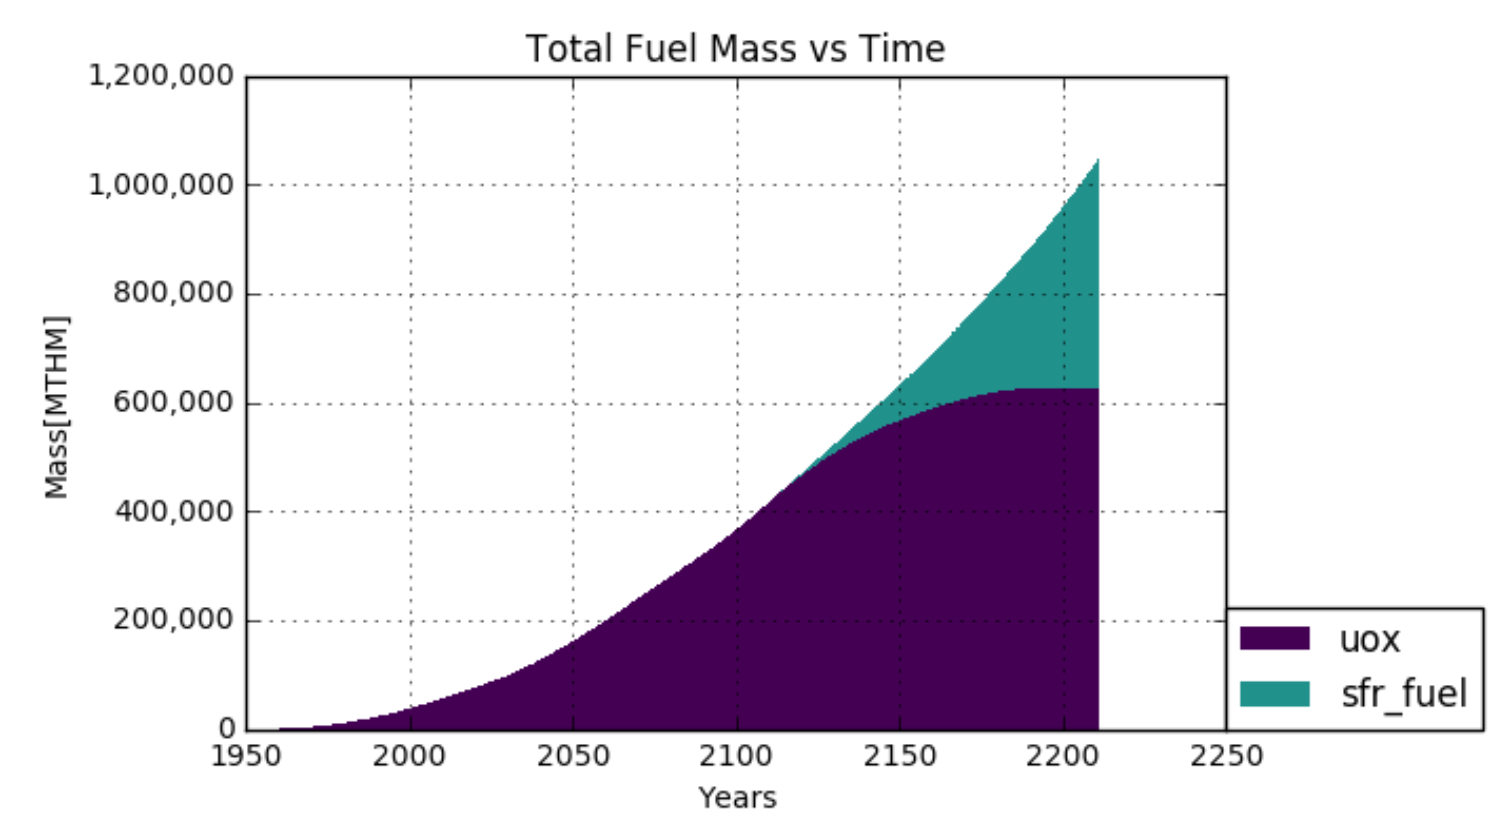
\includegraphics[width=\linewidth]{images/transition-fuelmass}
	\caption{Mass of fuel types over time in EG01-EG24 transition scenario.}
	\label{fig:fuel-mass}
\end{figure}